\section{Vergleich Simulation und Realität}
Um die Realitätsnähe der Simulation zu quantifizieren, wird der Ansatz über die Analyse von Aufnahmen diverser real
durchgeführter Stösse verfolgt. Dabei ist die Geschwindigkeit, welche die Kugel zu Beginn durch den Queue erfährt,
unbekannt. Diese wird in einem ersten Schritt eruiert. Bekannt dabei ist die Zeit sowie die Distanz, welche über die
Selektion einzelner Frames berechnet werden. Die Zeit ergibt sich durch den Abstand zweier Frames. Bei einem Video mit
30 FPS liegt der Fehler bei $\frac{1}{30} t [s] = 0.03 [s]$. Die Distanz wird über zwei selektierte Pixelpositionen
auf denselben Frames zur Berechnung der Zeit bestimmt. Diese Positionen werden zu Modellkoordinaten $P_0, P_1$
übersetzt\cite{project2:pixel_to_model_coordinates}, um die
Distanz in der Einheit $[mm]$ anzugeben. Anschliessend kann über die Formel \ref{eq:simvsReal:initialVelocity} die Anfangsgeschwindigkeit berechnet
werden, wobei auch die Gleitreibung $\mu_g$ sowie die Rollreibung $\mu_r$ bekannt sein müssen\footnote{Die Herleitung
erfolgt in Kapitel \ref{anhang:herleitung:initialVelocityWithTime}.}.
\begin{align}
    v_0^2 \cdot \frac{2 \cdot (\mu_g - \mu_r)}{49 \cdot g \cdot \mu_g^2} + v_0 \cdot \frac{t \cdot (2 \cdot \mu_r + 5 \cdot \mu_g)}{7 \cdot \mu_g} - \frac{1}{2} \cdot g \cdot \mu_r \cdot t^2 - s = 0\label{eq:simvsReal:initialVelocity}
\end{align}

Es wird eine quadratische Formel gelöst, welche zwei Resultate $v^1_0, v^2_0$ liefert. Von diesen wird nur die
kleinste positive Lösung $v_0$ in Betracht gezogen.

Sobald $v_0$ bestimmt ist, kann der Geschwindigkeitsvektor $\vec{v_0}$ berechnet werden. Dies geschieht über den Einheitsvektor,
welcher über die beiden Punkte zur Bestimmung der Distanz gegeben ist:
\begin{align}
    \vec{d} = P_1 - P_0\\
    \hat{d} = \frac{\vec{d}}{\norm{\vec{d}}}\\
    \vec{v_0} = v_0 \cdot \hat{d}
\end{align}

Im nächsten Schritt kann die Simulation mit der errechneten Startgeschwindigkeit des Spielballs ausgeführt werden.
Daraus resultiert eine Abfolge von Ereignissen, die in der Simulation gefunden wurden.
Diese werden mit manuell erstellten Ereignissabfolgen abgeglichen, bei welchem alle Positionen der Kugeln und Ereigniszeitpunkte
anhand der Videoaufnahmen bestimmt wurden. Die Summe der Differenzen zwischen den erwarteten Zeiten und Positionen bilden den Gesamtfehler.

\newpage
\subsection{Vergleich Bandenstoss}
Dieses Kapitel widmet sich dem Abgleich des erwarteten Verhaltens bei einer Bandenkollision wie in
Abschnitt \ref{kandidatensuche:bandenkollisionstheorie} beschrieben und dem effektiven Verhalten des verwendeten Tisches.
Es wird in zwei Subkapitel gegliedert, wobei sich das Erste mit der Beschreibung der Realität befasst, das Zweite hingegen
mit der Diskussion der Resultate.

\subsubsection{Bandenkollisionsrealität}
Es folgt die Beschreibung eines experimentellen Vorgehens, um zu prüfen, ob die Banden des verwendeten Billardtisches den
bekannten theoretischen und praktischen Vorgaben entsprechen. Dafür wurden zwei Videos aufgenommen und analysiert,
die einen schwächeren und einen starken Stoss zeigen.
Nach der beschriebenen Theorie müsste der Ausfallswinkel in etwa dem Einfallswinkel entsprechen.
Um einen Anhaltspunkt zu gewinnen, wurde ein Stoss
über eine Bande gesucht. Dadurch werden Linien auf den Tisch projiziert, die die Ausführung des Experiments vereinfachen.
Die angestossene Kugel müsste den visualisierten Linien folgen, sollte die Theorie auf den verwendeten Billardtisch
anwendbar sein.

Beim nachfolgend präsentierten schwachen Stoss in Abbildung \ref{fig:kugelverlauf_nach_bandenkollision_mit_schwachem_stoss_pool} wird erwartet, dass der Ausfallswinkel gemäss dem Prinzip 6.7 aus
Abschnitt \ref{kandidatensuche:bandenkollisionstheorie} grösser ausfällt. Dem ist effektiv so, jedoch ist
der Ausfallswinkel viel zu gross und kommt nicht durch den beschriebenen Topspin zustande, da die Kugel zu Beginn
eigentlich durchaus dem theoretischen Ausfallsweg folgen sollte. In Abbildung \ref{fig:rebound_angle_no_spin_slow_shot} sind
einzelne Frames des Stosses ersichtlich. Bis zum Bandenaufprall folg die weisse Kugel dem erwarteten Pfad. Bereits nach
dem Bandenaufprall in $f$ kann eine leichte seitliche Verschiebung der Kugel erkannt werden, welche den weiteren Verlauf
stark beeinflusst.

\begin{figure}[h!]
    \centering
    \begin{subfigure}[b]{0.2\textwidth}
        \centering
        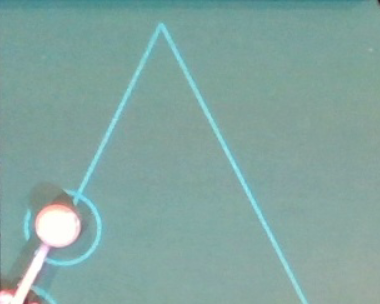
\includegraphics[width=1.0\linewidth]{../common/04_results/resources/simulation/rebound_angle_slow_pool/00_rail_rebound_angle_slow_pool_01.png}
        \caption{Ausfallswinkel bei schwachem Stoss in Pool - 1}
        \label{fig:rebound_angle_slow_pool_1}
    \end{subfigure}
    \hfill
    \begin{subfigure}[b]{0.2\textwidth}
        \centering
        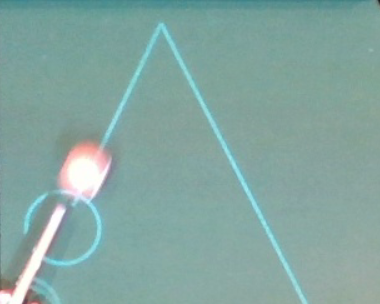
\includegraphics[width=1.0\linewidth]{../common/04_results/resources/simulation/rebound_angle_slow_pool/00_rail_rebound_angle_slow_pool_02.png}
        \caption{Ausfallswinkel bei schwachem Stoss in Pool - 2}
        \label{fig:rebound_angle_slow_pool_2}
    \end{subfigure}
    \hfill
    \begin{subfigure}[b]{0.2\textwidth}
        \centering
        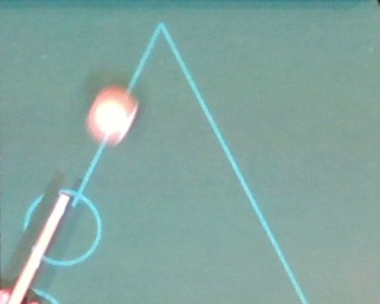
\includegraphics[width=1.0\linewidth]{../common/04_results/resources/simulation/rebound_angle_slow_pool/00_rail_rebound_angle_slow_pool_03.png}
        \caption{Ausfallswinkel bei schwachem Stoss in Pool - 3}
        \label{fig:rebound_angle_slow_pool_3}
    \end{subfigure}
    \hfill
    \begin{subfigure}[b]{0.2\textwidth}
        \centering
        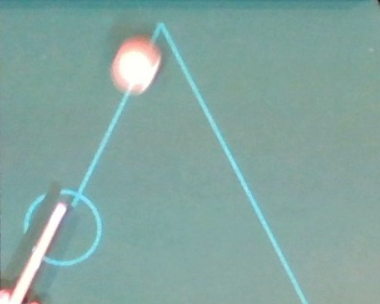
\includegraphics[width=1.0\linewidth]{../common/04_results/resources/simulation/rebound_angle_slow_pool/00_rail_rebound_angle_slow_pool_04.png}
        \caption{Ausfallswinkel bei schwachem Stoss in Pool - 4}
        \label{fig:rebound_angle_slow_pool_4}
    \end{subfigure}
    \hfill
    \begin{subfigure}[b]{0.2\textwidth}
        \centering
        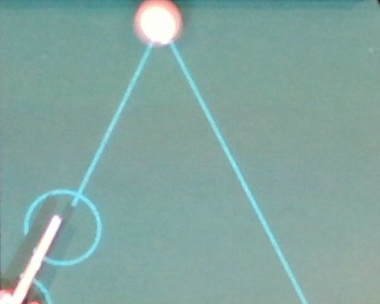
\includegraphics[width=1.0\linewidth]{../common/04_results/resources/simulation/rebound_angle_slow_pool/00_rail_rebound_angle_slow_pool_05.png}
        \caption{Ausfallswinkel bei schwachem Stoss in Pool - 5}
        \label{fig:rebound_angle_slow_pool_5}
    \end{subfigure}
    \hfill
    \begin{subfigure}[b]{0.2\textwidth}
        \centering
        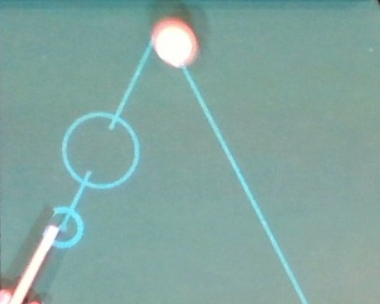
\includegraphics[width=1.0\linewidth]{../common/04_results/resources/simulation/rebound_angle_slow_pool/00_rail_rebound_angle_slow_pool_06.png}
        \caption{Ausfallswinkel bei schwachem Stoss in Pool - 6}
        \label{fig:rebound_angle_slow_pool_6}
    \end{subfigure}
    \hfill
    \begin{subfigure}[b]{0.2\textwidth}
        \centering
        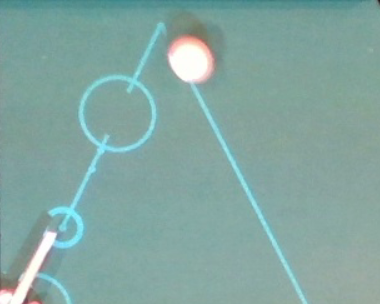
\includegraphics[width=1.0\linewidth]{../common/04_results/resources/simulation/rebound_angle_slow_pool/00_rail_rebound_angle_slow_pool_07.png}
        \caption{Ausfallswinkel bei schwachem Stoss in Pool - 7}
        \label{fig:rebound_angle_slow_pool_7}
    \end{subfigure}
    \hfill
    \begin{subfigure}[b]{0.2\textwidth}
        \centering
        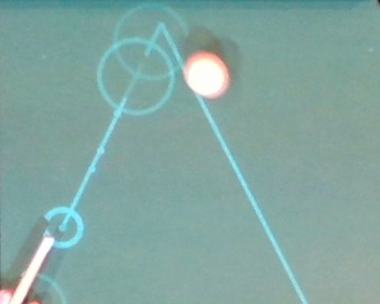
\includegraphics[width=1.0\linewidth]{../common/04_results/resources/simulation/rebound_angle_slow_pool/00_rail_rebound_angle_slow_pool_08.png}
        \caption{Ausfallswinkel bei schwachem Stoss in Pool - 8}
        \label{fig:rebound_angle_slow_pool_8}
    \end{subfigure}
    \hfill
    \begin{subfigure}[b]{0.2\textwidth}
        \centering
        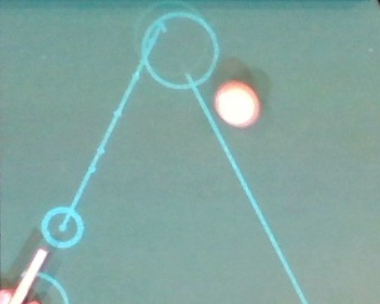
\includegraphics[width=1.0\linewidth]{../common/04_results/resources/simulation/rebound_angle_slow_pool/00_rail_rebound_angle_slow_pool_09.png}
        \caption{Ausfallswinkel bei schwachem Stoss in Pool - 9}
        \label{fig:rebound_angle_slow_pool_9}
    \end{subfigure}
    \hfill
    \begin{subfigure}[b]{0.2\textwidth}
        \centering
        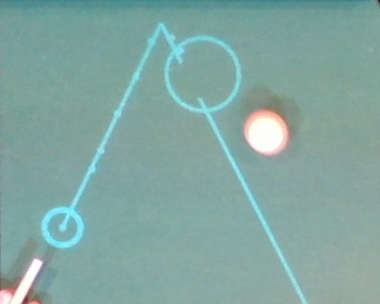
\includegraphics[width=1.0\linewidth]{../common/04_results/resources/simulation/rebound_angle_slow_pool/00_rail_rebound_angle_slow_pool_10.png}
        \caption{Ausfallswinkel bei schwachem Stoss in Pool - 10}
        \label{fig:rebound_angle_slow_pool_10}
    \end{subfigure}
    \hfill
    \begin{subfigure}[b]{0.2\textwidth}
        \centering
        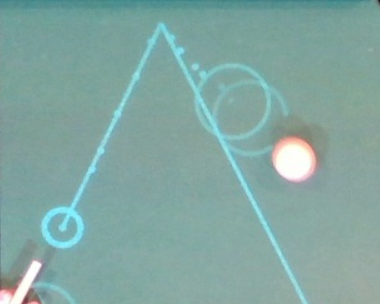
\includegraphics[width=1.0\linewidth]{../common/04_results/resources/simulation/rebound_angle_slow_pool/00_rail_rebound_angle_slow_pool_11.png}
        \caption{Ausfallswinkel bei schwachem Stoss in Pool - 11}
        \label{fig:rebound_angle_slow_pool_11}
    \end{subfigure}
    \hfill
    \begin{subfigure}[b]{0.2\textwidth}
        \centering
        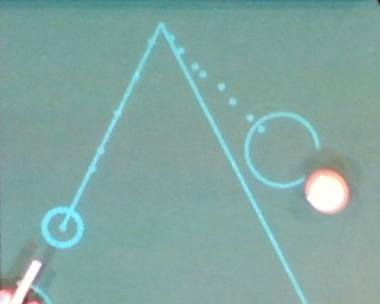
\includegraphics[width=1.0\linewidth]{../common/04_results/resources/simulation/rebound_angle_slow_pool/00_rail_rebound_angle_slow_pool_12.png}
        \caption{Ausfallswinkel bei schwachem Stoss in Pool - 12}
        \label{fig:rebound_angle_slow_pool_12}
    \end{subfigure}
    \caption{Kugelverlauf nach Bandenkollision mit schwachem Stoss - Pool}
    \label{fig:kugelverlauf_nach_bandenkollision_mit_schwachem_stoss_pool}
\end{figure}

Der starke Stoss wird in Abbildung \ref{fig:kugelverlauf_nach_bandenkollision_mit_starkem_stoss_pool} thematisiert.
Erwartet wird nach dem Prinzip 6.6 aus Kapitel \ref{kandidatensuche:bandenkollisionstheorie} ein kleinerer Ausfallswinkel als der Eingezeichnete.
Effektiv resultiert aber auch in diesem Fall wie im vorherig beschriebenen Fall ein grösserer Ausfallswinkel.
Nach dem Bandenaufprall in $f$ kann ebenso wieder eine leichte Versetzung der Kugel ausgemacht werden, die einen
grossen Einfluss hat.

\begin{figure}[h!]
    \centering
    \begin{subfigure}[b]{0.2\textwidth}
        \centering
        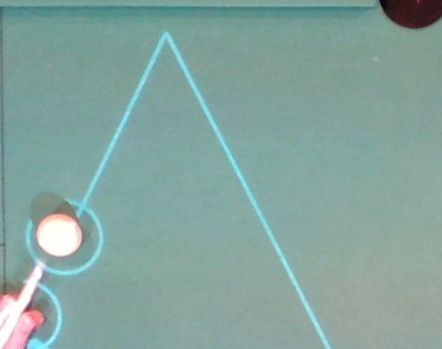
\includegraphics[width=1.0\linewidth]{../common/04_results/resources/simulation/rebound_angle_fast_pool/00_rail_rebound_angle_fast_pool_01.png}
        \caption{Ausfallswinkel bei starkem Stoss in Pool - 1}
        \label{fig:rebound_angle_fast_pool_1}
    \end{subfigure}
    \hfill
    \begin{subfigure}[b]{0.2\textwidth}
        \centering
        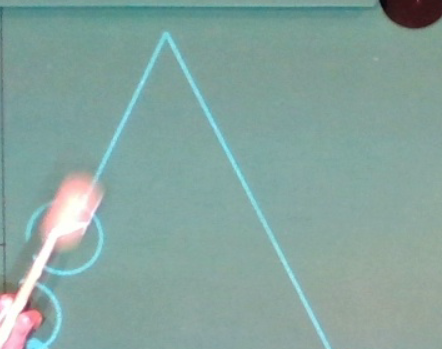
\includegraphics[width=1.0\linewidth]{../common/04_results/resources/simulation/rebound_angle_fast_pool/00_rail_rebound_angle_fast_pool_02.png}
        \caption{Ausfallswinkel bei starkem Stoss in Pool - 2}
        \label{fig:rebound_angle_fast_pool_2}
    \end{subfigure}
    \hfill
    \begin{subfigure}[b]{0.2\textwidth}
        \centering
        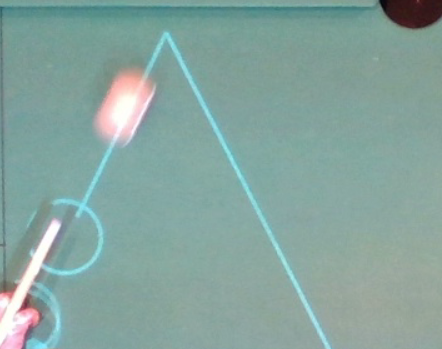
\includegraphics[width=1.0\linewidth]{../common/04_results/resources/simulation/rebound_angle_fast_pool/00_rail_rebound_angle_fast_pool_03.png}
        \caption{Ausfallswinkel bei starkem Stoss in Pool - 3}
        \label{fig:rebound_angle_fast_pool_3}
    \end{subfigure}
    \hfill
    \begin{subfigure}[b]{0.2\textwidth}
        \centering
        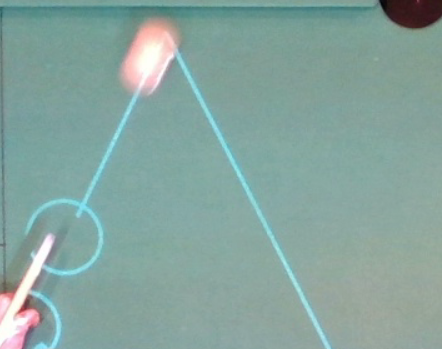
\includegraphics[width=1.0\linewidth]{../common/04_results/resources/simulation/rebound_angle_fast_pool/00_rail_rebound_angle_fast_pool_04.png}
        \caption{Ausfallswinkel bei starkem Stoss in Pool - 4}
        \label{fig:rebound_angle_fast_pool_4}
    \end{subfigure}
    \hfill
    \begin{subfigure}[b]{0.2\textwidth}
        \centering
        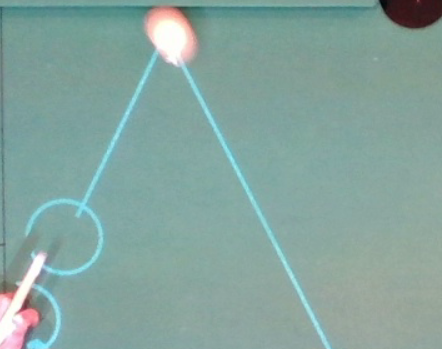
\includegraphics[width=1.0\linewidth]{../common/04_results/resources/simulation/rebound_angle_fast_pool/00_rail_rebound_angle_fast_pool_05.png}
        \caption{Ausfallswinkel bei starkem Stoss in Pool - 5}
        \label{fig:rebound_angle_fast_pool_5}
    \end{subfigure}
    \hfill
    \begin{subfigure}[b]{0.2\textwidth}
        \centering
        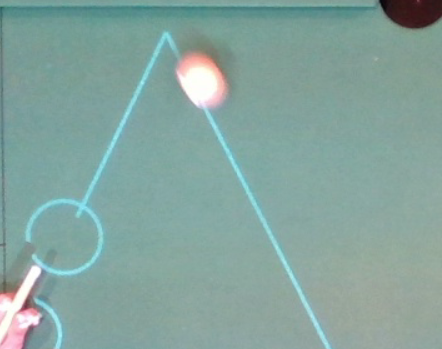
\includegraphics[width=1.0\linewidth]{../common/04_results/resources/simulation/rebound_angle_fast_pool/00_rail_rebound_angle_fast_pool_06.png}
        \caption{Ausfallswinkel bei starkem Stoss in Pool - 6}
        \label{fig:rebound_angle_fast_pool_6}
    \end{subfigure}
    \hfill
    \begin{subfigure}[b]{0.2\textwidth}
        \centering
        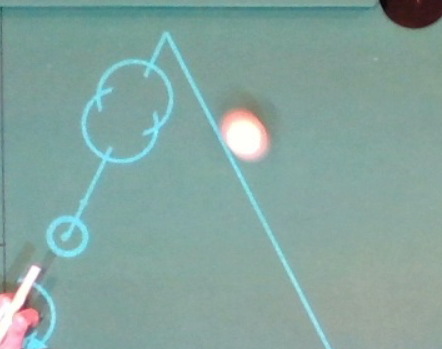
\includegraphics[width=1.0\linewidth]{../common/04_results/resources/simulation/rebound_angle_fast_pool/00_rail_rebound_angle_fast_pool_07.png}
        \caption{Ausfallswinkel bei starkem Stoss in Pool - 7}
        \label{fig:rebound_angle_fast_pool_7}
    \end{subfigure}
    \hfill
    \begin{subfigure}[b]{0.2\textwidth}
        \centering
        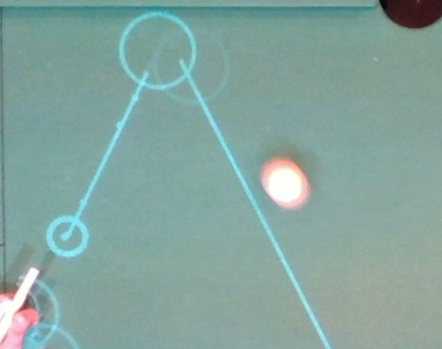
\includegraphics[width=1.0\linewidth]{../common/04_results/resources/simulation/rebound_angle_fast_pool/00_rail_rebound_angle_fast_pool_08.png}
        \caption{Ausfallswinkel bei starkem Stoss in Pool - 8}
        \label{fig:rebound_angle_fast_pool_8}
    \end{subfigure}
    \hfill
    \begin{subfigure}[b]{0.2\textwidth}
        \centering
        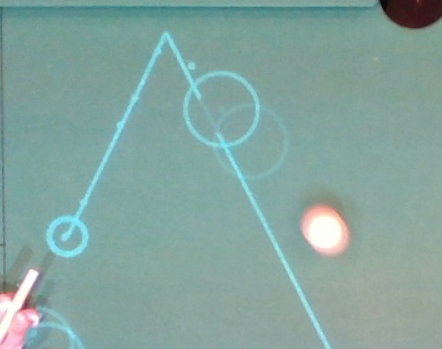
\includegraphics[width=1.0\linewidth]{../common/04_results/resources/simulation/rebound_angle_fast_pool/00_rail_rebound_angle_fast_pool_09.png}
        \caption{Ausfallswinkel bei starkem Stoss in Pool - 9}
        \label{fig:rebound_angle_fast_pool_9}
    \end{subfigure}
    \hfill
    \begin{subfigure}[b]{0.2\textwidth}
        \centering
        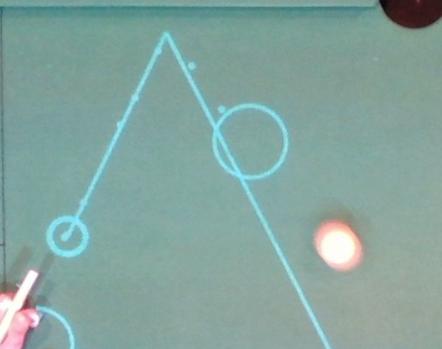
\includegraphics[width=1.0\linewidth]{../common/04_results/resources/simulation/rebound_angle_fast_pool/00_rail_rebound_angle_fast_pool_10.png}
        \caption{Ausfallswinkel bei starkem Stoss in Pool - 10}
        \label{fig:rebound_angle_fast_pool_10}
    \end{subfigure}
    \hfill
    \begin{subfigure}[b]{0.2\textwidth}
        \centering
        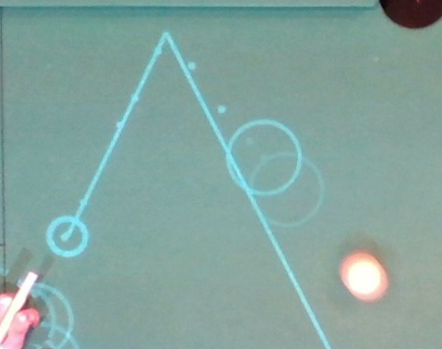
\includegraphics[width=1.0\linewidth]{../common/04_results/resources/simulation/rebound_angle_fast_pool/00_rail_rebound_angle_fast_pool_11.png}
        \caption{Ausfallswinkel bei starkem Stoss in Pool - 11}
        \label{fig:rebound_angle_fast_pool_11}
    \end{subfigure}
    \hfill
    \begin{subfigure}[b]{0.2\textwidth}
        \centering
        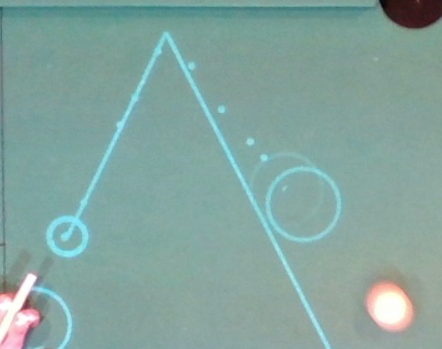
\includegraphics[width=1.0\linewidth]{../common/04_results/resources/simulation/rebound_angle_fast_pool/00_rail_rebound_angle_fast_pool_12.png}
        \caption{Ausfallswinkel bei starkem Stoss in Pool - 12}
        \label{fig:rebound_angle_fast_pool_12}
    \end{subfigure}
    \caption{Kugelverlauf nach Bandenkollision mit starkem Stoss - Pool}
    \label{fig:kugelverlauf_nach_bandenkollision_mit_starkem_stoss_pool}
\end{figure}

\newpage
Weiterhin werden anstelle der grösseren Pool-Kugeln kleinere Snooker-Kugeln verwendet. Dies kann ebenfalls einen
Einfluss auf das Zusammenspiel mit der Bande haben. Daher wurden dieselben Experimente, wie sie in diesem Kapitel vorgängig beschrieben
wurden, ebenfalls für Snooker-Kugeln durchgeführt, was den Abbildungen \ref{fig:kugelverlauf_nach_bandenkollision_mit_schwachem_stoss_snooker}
und \ref{fig:kugelverlauf_nach_bandenkollision_mit_starkem_stoss_snooker} zu entnehmen ist.
Das Verhalten ist im Wesentlichen dasselbe, der Ausfallswinkel ist in beiden Fällen viel zu gross.

\begin{figure}[h!]
    \centering
    \begin{subfigure}[b]{0.2\textwidth}
        \centering
        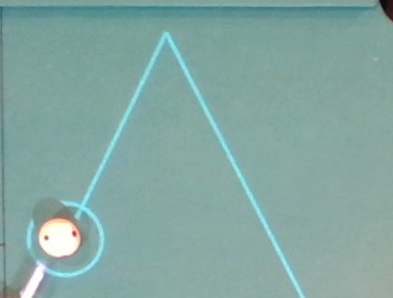
\includegraphics[width=1.0\linewidth]{../common/04_results/resources/simulation/rebound_angle_slow_snooker/00_rail_rebound_angle_slow_snooker_01.png}
        \caption{Ausfallswinkel bei schwachem Stoss in Snooker - 1}
        \label{fig:rebound_angle_slow_snooker_1}
    \end{subfigure}
    \hfill
    \begin{subfigure}[b]{0.2\textwidth}
        \centering
        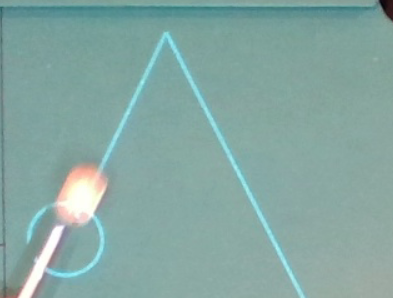
\includegraphics[width=1.0\linewidth]{../common/04_results/resources/simulation/rebound_angle_slow_snooker/00_rail_rebound_angle_slow_snooker_02.png}
        \caption{Ausfallswinkel bei schwachem Stoss in Snooker - 2}
        \label{fig:rebound_angle_slow_snooker_2}
    \end{subfigure}
    \hfill
    \begin{subfigure}[b]{0.2\textwidth}
        \centering
        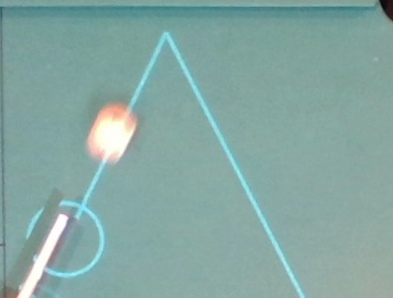
\includegraphics[width=1.0\linewidth]{../common/04_results/resources/simulation/rebound_angle_slow_snooker/00_rail_rebound_angle_slow_snooker_03.png}
        \caption{Ausfallswinkel bei schwachem Stoss in Snooker - 3}
        \label{fig:rebound_angle_slow_snooker_3}
    \end{subfigure}
    \hfill
    \begin{subfigure}[b]{0.2\textwidth}
        \centering
        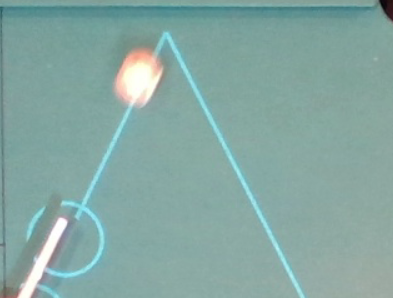
\includegraphics[width=1.0\linewidth]{../common/04_results/resources/simulation/rebound_angle_slow_snooker/00_rail_rebound_angle_slow_snooker_04.png}
        \caption{Ausfallswinkel bei schwachem Stoss in Snooker - 4}
        \label{fig:rebound_angle_slow_snooker_4}
    \end{subfigure}
    \hfill
    \begin{subfigure}[b]{0.2\textwidth}
        \centering
        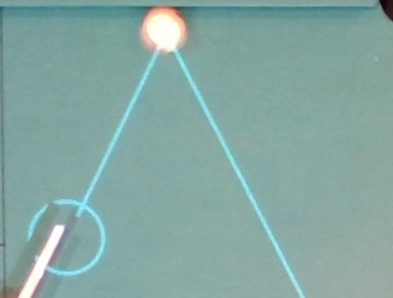
\includegraphics[width=1.0\linewidth]{../common/04_results/resources/simulation/rebound_angle_slow_snooker/00_rail_rebound_angle_slow_snooker_05.png}
        \caption{Ausfallswinkel bei schwachem Stoss in Snooker - 5}
        \label{fig:rebound_angle_slow_snooker_5}
    \end{subfigure}
    \hfill
    \begin{subfigure}[b]{0.2\textwidth}
        \centering
        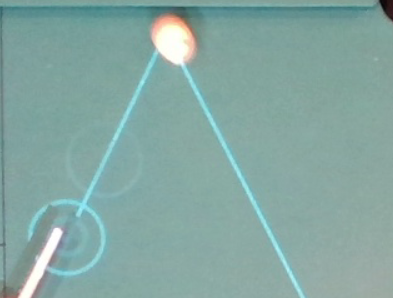
\includegraphics[width=1.0\linewidth]{../common/04_results/resources/simulation/rebound_angle_slow_snooker/00_rail_rebound_angle_slow_snooker_06.png}
        \caption{Ausfallswinkel bei schwachem Stoss in Snooker - 6}
        \label{fig:rebound_angle_slow_snooker_6}
    \end{subfigure}
    \hfill
    \begin{subfigure}[b]{0.2\textwidth}
        \centering
        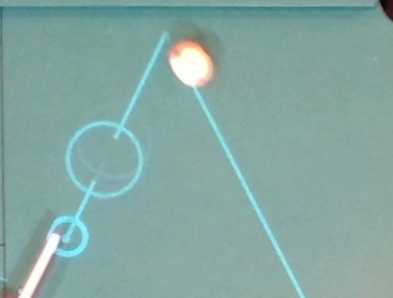
\includegraphics[width=1.0\linewidth]{../common/04_results/resources/simulation/rebound_angle_slow_snooker/00_rail_rebound_angle_slow_snooker_07.png}
        \caption{Ausfallswinkel bei schwachem Stoss in Snooker - 7}
        \label{fig:rebound_angle_slow_snooker_7}
    \end{subfigure}
    \hfill
    \begin{subfigure}[b]{0.2\textwidth}
        \centering
        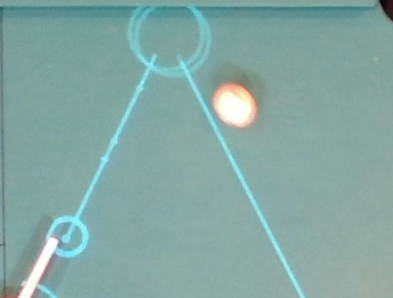
\includegraphics[width=1.0\linewidth]{../common/04_results/resources/simulation/rebound_angle_slow_snooker/00_rail_rebound_angle_slow_snooker_08.png}
        \caption{Ausfallswinkel bei schwachem Stoss in Snooker - 8}
        \label{fig:rebound_angle_slow_snooker_8}
    \end{subfigure}
    \hfill
    \begin{subfigure}[b]{0.2\textwidth}
        \centering
        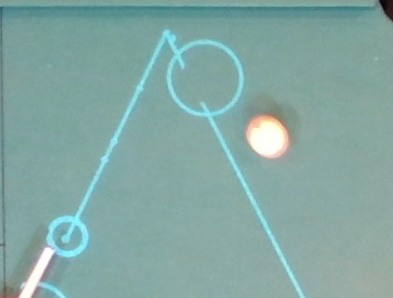
\includegraphics[width=1.0\linewidth]{../common/04_results/resources/simulation/rebound_angle_slow_snooker/00_rail_rebound_angle_slow_snooker_09.png}
        \caption{Ausfallswinkel bei schwachem Stoss in Snooker - 9}
        \label{fig:rebound_angle_slow_snooker_9}
    \end{subfigure}
    \hfill
    \begin{subfigure}[b]{0.2\textwidth}
        \centering
        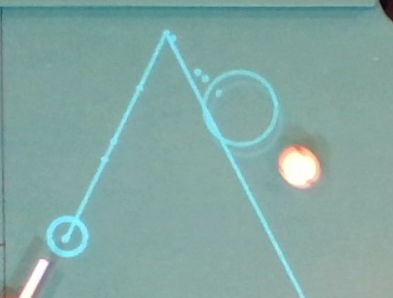
\includegraphics[width=1.0\linewidth]{../common/04_results/resources/simulation/rebound_angle_slow_snooker/00_rail_rebound_angle_slow_snooker_10.png}
        \caption{Ausfallswinkel bei schwachem Stoss in Snooker - 10}
        \label{fig:rebound_angle_slow_snooker_10}
    \end{subfigure}
    \hfill
    \begin{subfigure}[b]{0.2\textwidth}
        \centering
        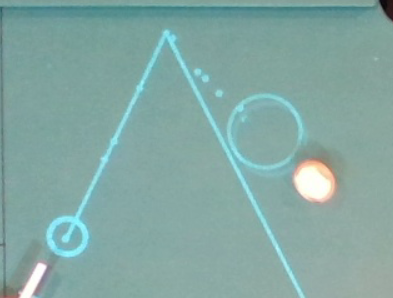
\includegraphics[width=1.0\linewidth]{../common/04_results/resources/simulation/rebound_angle_slow_snooker/00_rail_rebound_angle_slow_snooker_11.png}
        \caption{Ausfallswinkel bei schwachem Stoss in Snooker - 11}
        \label{fig:rebound_angle_slow_snooker_11}
    \end{subfigure}
    \hfill
    \begin{subfigure}[b]{0.2\textwidth}
        \centering
        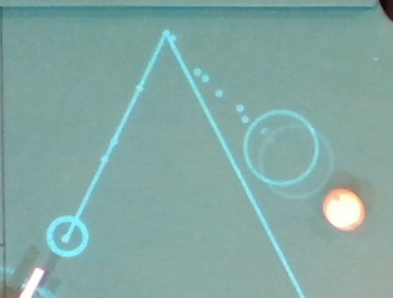
\includegraphics[width=1.0\linewidth]{../common/04_results/resources/simulation/rebound_angle_slow_snooker/00_rail_rebound_angle_slow_snooker_12.png}
        \caption{Ausfallswinkel bei schwachem Stoss in Snooker - 12}
        \label{fig:rebound_angle_slow_snooker_12}
    \end{subfigure}
    \caption{Kugelverlauf nach Bandenkollision mit schwachem Stoss - Snooker}
    \label{fig:kugelverlauf_nach_bandenkollision_mit_schwachem_stoss_snooker}
\end{figure}

\begin{figure}[h!]
    \centering
    \begin{subfigure}[b]{0.2\textwidth}
        \centering
        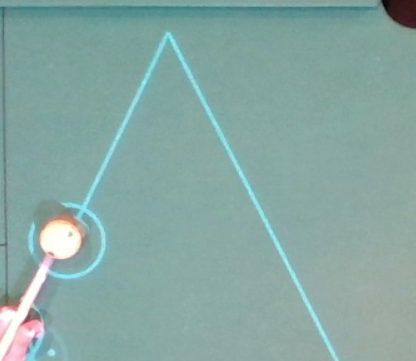
\includegraphics[width=1.0\linewidth]{../common/04_results/resources/simulation/rebound_angle_fast_snooker/00_rail_rebound_angle_fast_snooker_01.png}
        \caption{Ausfallswinkel bei starkem Stoss in Snooker - 1}
        \label{fig:rebound_angle_fast_snooker_1}
    \end{subfigure}
    \hfill
    \begin{subfigure}[b]{0.2\textwidth}
        \centering
        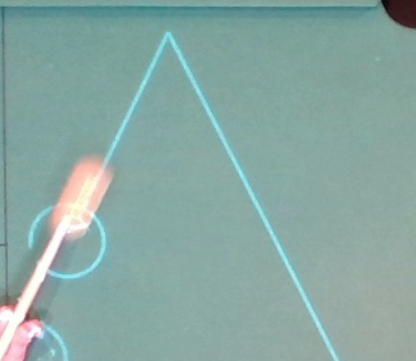
\includegraphics[width=1.0\linewidth]{../common/04_results/resources/simulation/rebound_angle_fast_snooker/00_rail_rebound_angle_fast_snooker_02.png}
        \caption{Ausfallswinkel bei starkem Stoss in Snooker - 2}
        \label{fig:rebound_angle_fast_snooker_2}
    \end{subfigure}
    \hfill
    \begin{subfigure}[b]{0.2\textwidth}
        \centering
        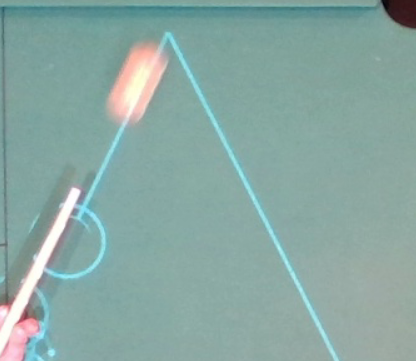
\includegraphics[width=1.0\linewidth]{../common/04_results/resources/simulation/rebound_angle_fast_snooker/00_rail_rebound_angle_fast_snooker_03.png}
        \caption{Ausfallswinkel bei starkem Stoss in Snooker - 3}
        \label{fig:rebound_angle_fast_snooker_3}
    \end{subfigure}
    \hfill
    \begin{subfigure}[b]{0.2\textwidth}
        \centering
        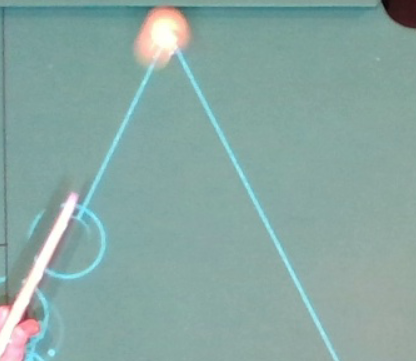
\includegraphics[width=1.0\linewidth]{../common/04_results/resources/simulation/rebound_angle_fast_snooker/00_rail_rebound_angle_fast_snooker_04.png}
        \caption{Ausfallswinkel bei starkem Stoss in Snooker - 4}
        \label{fig:rebound_angle_fast_snooker_4}
    \end{subfigure}
    \hfill
    \begin{subfigure}[b]{0.2\textwidth}
        \centering
        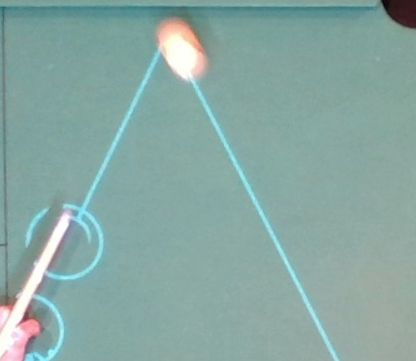
\includegraphics[width=1.0\linewidth]{../common/04_results/resources/simulation/rebound_angle_fast_snooker/00_rail_rebound_angle_fast_snooker_05.png}
        \caption{Ausfallswinkel bei starkem Stoss in Snooker - 5}
        \label{fig:rebound_angle_fast_snooker_5}
    \end{subfigure}
    \hfill
    \begin{subfigure}[b]{0.2\textwidth}
        \centering
        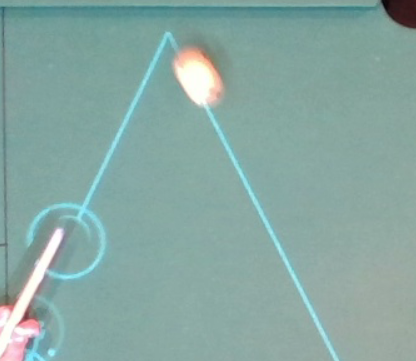
\includegraphics[width=1.0\linewidth]{../common/04_results/resources/simulation/rebound_angle_fast_snooker/00_rail_rebound_angle_fast_snooker_06.png}
        \caption{Ausfallswinkel bei starkem Stoss in Snooker - 6}
        \label{fig:rebound_angle_fast_snooker_6}
    \end{subfigure}
    \hfill
    \begin{subfigure}[b]{0.2\textwidth}
        \centering
        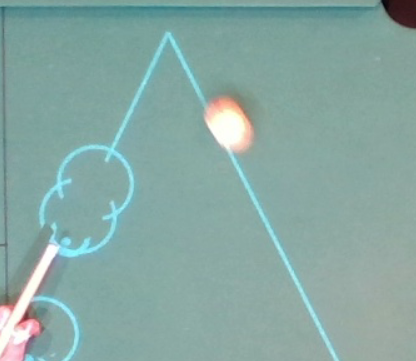
\includegraphics[width=1.0\linewidth]{../common/04_results/resources/simulation/rebound_angle_fast_snooker/00_rail_rebound_angle_fast_snooker_07.png}
        \caption{Ausfallswinkel bei starkem Stoss in Snooker - 7}
        \label{fig:rebound_angle_fast_snooker_7}
    \end{subfigure}
    \hfill
    \begin{subfigure}[b]{0.2\textwidth}
        \centering
        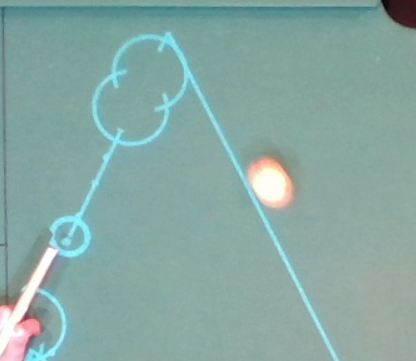
\includegraphics[width=1.0\linewidth]{../common/04_results/resources/simulation/rebound_angle_fast_snooker/00_rail_rebound_angle_fast_snooker_08.png}
        \caption{Ausfallswinkel bei starkem Stoss in Snooker - 8}
        \label{fig:rebound_angle_fast_snooker_8}
    \end{subfigure}
    \hfill
    \begin{subfigure}[b]{0.2\textwidth}
        \centering
        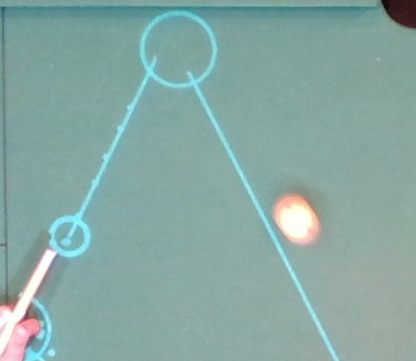
\includegraphics[width=1.0\linewidth]{../common/04_results/resources/simulation/rebound_angle_fast_snooker/00_rail_rebound_angle_fast_snooker_09.png}
        \caption{Ausfallswinkel bei starkem Stoss in Snooker - 9}
        \label{fig:rebound_angle_fast_snooker_9}
    \end{subfigure}
    \hfill
    \begin{subfigure}[b]{0.2\textwidth}
        \centering
        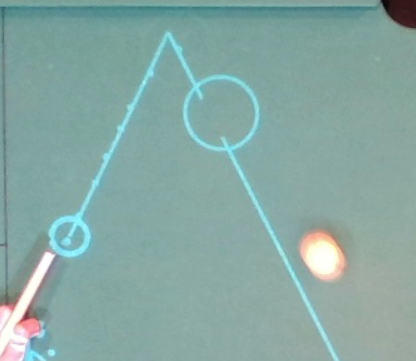
\includegraphics[width=1.0\linewidth]{../common/04_results/resources/simulation/rebound_angle_fast_snooker/00_rail_rebound_angle_fast_snooker_10.png}
        \caption{Ausfallswinkel bei starkem Stoss in Snooker - 10}
        \label{fig:rebound_angle_fast_snooker_10}
    \end{subfigure}
    \hfill
    \begin{subfigure}[b]{0.2\textwidth}
        \centering
        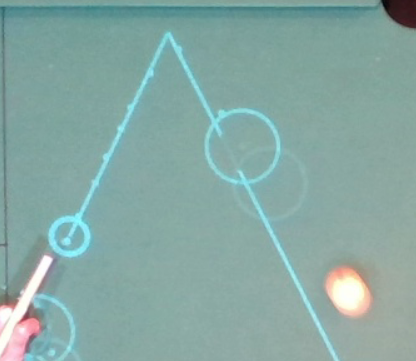
\includegraphics[width=1.0\linewidth]{../common/04_results/resources/simulation/rebound_angle_fast_snooker/00_rail_rebound_angle_fast_snooker_11.png}
        \caption{Ausfallswinkel bei starkem Stoss in Snooker - 11}
        \label{fig:rebound_angle_fast_snooker_11}
    \end{subfigure}
    \hfill
    \begin{subfigure}[b]{0.2\textwidth}
        \centering
        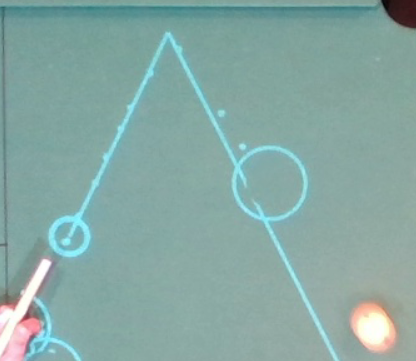
\includegraphics[width=1.0\linewidth]{../common/04_results/resources/simulation/rebound_angle_fast_snooker/00_rail_rebound_angle_fast_snooker_12.png}
        \caption{Ausfallswinkel bei starkem Stoss in Snooker - 12}
        \label{fig:rebound_angle_fast_snooker_12}
    \end{subfigure}
    \caption{Kugelverlauf nach Bandenkollision mit starkem Stoss - Snooker}
    \label{fig:kugelverlauf_nach_bandenkollision_mit_starkem_stoss_snooker}
\end{figure}

\newpage
An dieser Stelle kann festgehalten werden, dass die Bande des Billardtisches nicht die erwarteten Eigenschaften
aufweist, was wahrscheinlich daran liegt, dass es ein sehr günstig erhältliches Produkt und dementsprechend auch
die Qualität ist. Anzumerken ist, dass während dem Spielen aufgefallen ist, dass das rechte Bandensegment die
Eigenschaften besser erfüllt. Festgehalten wird auch die Tatsache, dass das Verwenden der Snooker-Kugeln einen
Einfluss haben kann, dieser aber nicht so stark ins Gewicht fällt wie das grundlegende Fehlverhalten
der Bande.

% TODO: Bandentest in Realität durchführen
Dass die Banden nicht in Ordnung sind, zeigt ein weiterer durchgeführter Test. Demnach muss eine Kugel insgesamt vier Mal über
die Tischlänge oder fünf Mal über die Tischbreite laufen, wenn sie stark angespielt wird\cite{sport64:bandengummi}.
Auf dem verwendeten Tisch schafft die Kugel nur deren TODO, respektive TODO Läufe.

\newpage
\subsubsection{Diskussion}
Nach dem Autor des Buches \glqq The illustrated principles of pool and billiards\grqq{} gibt es diverse Einflüsse,
die den Ausfallswinkel der Kugel nach einer Bandenkollision beeinträchtigen. Laut ihm ist daher eine mittlere
Geschwindigkeit zu bevorzugen, welche diese unerwünschten Effekte minimal hält\cite{book:the_ilustrated_principles_of_pool_and_billiards}.
Leider findet sich keine Aussage, wie stark ein schwacher, mittlerer oder starker Stoss genau ist.

Demgegenüber steht die Aussage der Autoren des Papers \glqq A theoretical analysis of billiard ball dynamics under cushion impacts\grqq, welche ebenfalls
gewisse Abweichungen festgestellt haben, jedoch im Schnitt durchaus einen linearen Zusammenhang feststellen konnten.

Einen Einfluss auf diese Untersuchungen hat die verwendete Hardware, namentlich der Billardtisch und die
zugehörigen Kugeln. So ist das Verhalten einer Kugel nach einer Bandenkollision vor allem vom verwendeten Gummi der
Bande abhängig. Dadurch kann es zu gewichtigen Unterschieden kommen.
Diese theoretischen und praktischen Erkenntnisse bilden dennoch die Grundlage in der vorliegenden Arbeit,
da davon ausgegangen werden kann, dass im professionellen  Umfeld ein Billardtisch diese genannten Eigenschaften aufweisen muss.

Leider gilt dies nicht für den in dieser Arbeit verwendeten Billardtisch.
Dessen Bandeneigenschaften entsprechen keinesfalls den Vorgaben und ist für den professionellen und privaten Gebrauch ungeeignet,
da wahrscheinlich ein günstiges Gummi verwendet wurde.
Ein entsprechendes Statement ist auch aus einer Bewertung aus dem Onlineshop zu entnehmen, siehe Abbildung \ref{fig:bewertung_billardtisch}.

\begin{figure}[h!]
    \begin{center}
        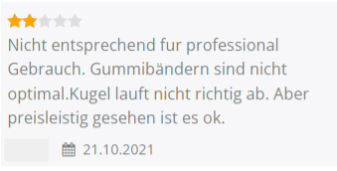
\includegraphics[width=0.3\linewidth]{../common/04_results/resources/simulation/00_bewertung_billardtisch.png}
    \end{center}
    \caption{Bewertung zu Billardtisch\cite{gonser:billardtisch}}
    \label{fig:bewertung_billardtisch}
\end{figure}

Demnach wird festgehalten, dass die in dieser Arbeit verwendete Theorie durchaus funktioniert und der Realität
standhält, im Zusammenhang mit dem verwendeten Billardtisch dennoch leider nicht verwendbar ist aufgrund der schlechten
Qualität desselbigen.
% TODO: vergleich ausschnitte vom video und simulation zu bestimmten Ereigniszeitpunkten für Diskussion über Weg der weissen Kugel
